\documentclass[language=french,style=exam]{smo}

\usepackage{tikz}

\title{SMO - Tour préliminaire}

\begin{document}

\begin{enumerate}

\item[\textbf{1.}] 
Dans la rue OSM, il y a $n$ maisons numérotées de 1 à $n$, où $n$ est un entier naturel. Les maisons avec un numéro impair se trouvent sur le côté gauche de la rue et celles avec un numéro pair sur le côté droit. La factrice Cunégonde souhaite apporter à chaque maison un journal. Combien a-t-elle de manières de le faire, si elle veut traverser la rue après avoir distribué chaque journal ?

\bigskip

\item[\textbf{2.}] 
Pour quels entiers naturels $n$ est-il possible de recouvrir un échiquier $n\times n$, sans trou et sans recouvrement, avec des T-Tetrominos et un nombre impair de Square-Tetrominos ?
\vspace{0.2cm}
\begin{center}
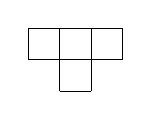
\begin{tikzpicture}[scale=0.4]
\draw (0,1) grid (3,2);
\draw (1,0) grid (2,1);
\end{tikzpicture}
\quad
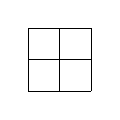
\begin{tikzpicture}[scale=0.4]
\draw (0,0) grid (2,2);
\end{tikzpicture}
\end{center}
\vspace{0.2cm}
\textit{Remarque: il est possible de n'utiliser aucun T-Tetromino.}
\vspace{0.2cm}
\item[\textbf{3.}]
Trouver tous les triplets $(a,b,c)$ d'entiers naturels tels que
\[
\frac{a+b}{c},\frac{b+c}{a},\frac{c+a}{b}
\]
%\[
%c \,|\, a+b \qquad a \,|\, b+c \qquad b \,|\, a+c
%\]
soient tous trois des nombres entiers.

\bigskip

\item[\textbf{4.}] 
Soit $ABC$ un triangle aigu et $W$ le point d'intersection de la bissectrice de l'angle $\angle ACB$ et du côté $AB$. Soient ensuite $I_A$ et $I_B$ les centres des cercles inscrits des triangles $AWC$ respectivement $WBC$. Les droites $I_AW$ et $I_BB$ se coupent en un point $D$. Soit $M$ le milieu du segment $DI_B$. Montrer que $MWBC$ est un quadrilatère inscrit.

\textit{Remarque: les trois bissectrices d'un triangle se coupent en un point, le centre du cercle inscrit.}

\bigskip

\item[\textbf{5.}] 
On appelle un \textit{escalier} la pièce représentée ci-dessous. Pour quelles paires de nombres naturels $(m,n)$, avec $m,n\geq 6$, est-il possible de recouvrir un échiquier $m\times n$ avec des escaliers, sans trou et sans recouvrement ?
\vspace{0.2cm}
\begin{center}

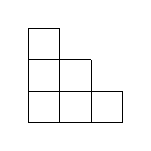
\begin{tikzpicture}[scale=0.4]
\draw (-1,0) grid (2,1);
\draw (-1,1) grid (1,2);
\draw (-1,2) grid (0,3);
\end{tikzpicture}
\quad
\end{center}

\bigskip

\end{enumerate}

\vspace{1cm}

\center{\hspace{1cm} Bonne chance!}
\end{document}
